\section{Propuesta de solución}
\label{sec:propuesta-sol} 
(Descripción de la propuesta para solucionar el problema)

La propuesta para detectar fuga de información en aplicaciones Android, antes de
su publicación, consiste en proveer al desarrollador una herramienta para
análisis estático de flujos de información de la aplicación. Así, partiendo de
las anotaciones de seguridad que el desarrollador defina en el código fuente, se
verifica si la aplicación cumple con políticas de seguridad.\newline
\textcolor{red}{Cómo sabe el desarrollador que información anota con nivel de
seguridad bajo y con nivel de seguridad alto?}\newline
Los requerimientos iniciales para construir tal herramienta son: un lenguaje
tipado de seguridad que permita anotar código fuente Android, y el conjunto de
reglas que evaluarán las políticas de confidencialidad.\newline 
Al consultar literatura científica al respecto, se encuentran herramientas como
JIF \ref{JIF-Tool} y JOANA \ref{JOANA-Tool}, especializadas en anotar código
Java, pero no código Android. Es decir, las anotaciones son válidas para clases
del lenguaje java estandar, pero no para clases específicas de la API de Android.

Si bien, ambas analizan flujos de información en aplicaciones Java, y
podrían ser extendidas para anotar código Android, las técnicas utilizadas por cada una
son diferentes, por un lado, JIF es un lenguaje tipado de seguridad que basa su
análisis en el chequeo de tipos. Por el otro, JOANA es un framework basado en
análisis de grafos de dependencia. Mientras JOANA se enfoca en precisión, JIF
posee un modelo de anotaciones (DLM) encargado de definir la lattice de
seguridad adecuada para las anotaciones en el código fuente, ofreciendo un
maduro sistema que además de evaluar políticas de confidencialidad, e
integridad, permite definir características de seguridad adicionales como
declasificación y endorsement.
Acorde a los propósitos del presente trabajo, JIF ofrece los beneficios de un
lenguaje tipado de seguridad y un sistema  sólido  de anotaciones, facilitando
la definición de las propiedades de seguridad a verificar.\newline 
Partiendo de JIF como el lenguaje tipado de seguridad, los retos subsiguientes
son: implementar el setup de JIF para Android e integrar un clasificador
para sources y sinks de Android. 
El setup de JIF para Android consiste en implementar adaptaciones necesarias
a las clases de la API de Android, de modo que el compilador de Jif las
reconozca, y sea posible adicionar anotaciones de Jif dentro de aplicaciones
Android. Puesto que, aunque Jif permite extender al lenguaje Java, y en el fondo
las clases de la API Android estan implementadas en Java, si no se cuenta con
una versión Jif de tales clases, el compilador de Jif no tiene como
reconocerlas, por tanto, no admite anotaciones en programas que usen esas
clases(aplicativos Android.)\newline
% en implementar las adaptaciones necesarias
% para que el lenguaje JIF reconozca código de la API de Android, y admita
% anotaciones JIF dentro de código Android, pues aunque en esencia el código
% Android es código Java, JIF no tiene como saberlo. 
Con la integración de un clasificador de sources y sinks para Android al sistema
de anotaciones de JIF, se provee información necesaria para construir las
políticas de seguridad. Puesto que, al conocer qué código de la Api de Android,
es considerado como source o como sink, se tiene el criterio para decidir su
anotación. Es decir, permiten conocer el nivel de seguridad con que deben ser
anotados el código tanto de la API como el código del aplicativo a
analizar.\newline
%Si el desarrollador no sabe que es source y que es sink, cómo sabe que nivel
% de seguridad anotar durante la implementación de la versión JIf que va a
% evaluar 
La figura \ref{fig:desingInteger} expone los elementos necesarios para construir la
herramienta de análisis.
Básicamente, se requiere un módulo que extienda las clases en JIF para que el
lenguaje reconozca código de la API Android(\emph{Android Jif Setup}), más un
módulo que integre el clasificador de sources y sinks para Android(\emph{Sources
y Sinks}). El clasificador permite conocer que código de la API de Android es
considerado como source o sink, dando las pautas para anotación del código
Android. Es decir, permiten conocer el nivel de seguridad con que deben ser
anotados el código tanto de la API como, el código del aplicativo a analizar.
Estos dos modulos deben tener comunicación con el módulo que evalúa las
políticas de seguridad \emph{verificador de políticas}, que en el esencia es el
compilador de Jif.\newline
% s decir, para que admita anotaciones dentro del código Android: Setup extended JIF classes.
% Un módulo que integre el clasificador de sources y sinks de Android al
% sistema de anotaciones en JIF:  Android Sources and Sinks. Adicionalmente, se
% requiere un modulo que evalúe las políticas de confidencialidad, Checking
% Rule Sets, que debe tener comunicación con los módulos anteriormente descritos.
Tal como ilustra la figura \ref{fig:desingInteger}, la entrada para la herramienta de
análisis debe ser el código fuente de la aplicación, debidamente anotado por el
desarrollador. De modo que el desarrollador defina las políticas de seguridad a
evaluar. A partir de tales anotaciones, la herramienta de análisis verifica si
los flujos de información del aplicativo, cumplen con la política de seguridad
expresada a través sus anotaciones.
Habiendo realizado las extensiones necesarias, se espera contar con una
herramienta de análisis de flujo de información, para aplicativos Android,
mediante el sistema de anotaciones de Jif.
\begin{figure}[t!]
	\begin{center}
	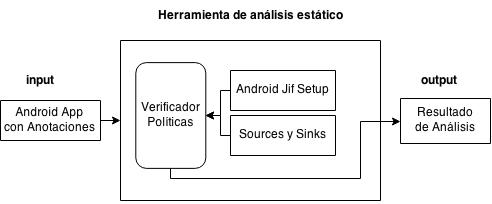
\includegraphics[width=10cm]{desing3-intergration.jpg}
	\end{center}
	\caption{Herramienta de análisis estático  }
	\label{fig:desingInteger}
\end{figure}

% \begin{figure}[t!]
% 	\begin{center}
% 	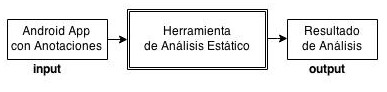
\includegraphics[width=9cm]{desingInOut-3.jpg}
% 	\end{center}
% 	\caption{Herramienta de análisis estático. Ilustra entradas y salidas
% 	esperadas}
% 	\label{fig:desing1}
% \end{figure} 

Luego, la estrategia de evaluación, consiste en verificar si la herramienta
implementada identifica pérdida de información mediante detección de flujos
implícitos. Esto debido a que, como se menciona en la descripción del problema,
parte importante de las propuestas para detección de fuga de información en
aplicaciones Android, hacen data-flow analysis aplicando técnicas de análisis
tainting, y en contraste con las técnicas de análisis de flujo de información,
las técnicas de análisis tainting no necesariamente consideran flujos
implícitos. Por tanto, al estar basada en JIF, cuyo enfoque de análisis es
precisamente flujo de información, se esperaría que la herramienta planteada
esté en capacidad de reconocer flujos implícitos.

% Se esperaría que: al realizar análisis de flujo de información aplicando
% técnicas Security-Typing, la herramienta propuesta, esté en capacidad de
% reconocer flujos implícitos.\newline
% Más específicamente, se puede tomar el conjunto de aplicaciones utilizadas como
% casos de prueba para la detección de flujos implícitos en
% DroidBench\cite{DroidBenchBenchmarks}, el benchmark de Flowdroid, y analizarlas
% con la herramienta propuesta.\newline

Más específicamente, se puede partir de DroidBench\cite{DroidBenchBenchmarks},
el benchmark de Flowdroid[\ref{FlowDroid-Tool}], tomar el conjunto de
aplicaciones con que prueban la detección de flujos implícitos, y analizarlas
con la herramienta propuesta.\newline
Finalmente estos resultados serían
comparados con los obtenidos mediante otras herramientas para análisis de fuga
de información en aplicaciones Android.\newline

En este orden de ideas, la evaluación de la herramienta propuesta está enfocada
en: medir recall frente a la detección de flujos implícitos, es decir, medir que
no genere falsos negativos ante la existencia de fugas de información,
provenientes de flujos implícitos.\newline







